
\documentclass{cccg16}

\usepackage{amssymb, amsmath}
\usepackage{graphicx}
\usepackage{hyperref}
\usepackage[utf8]{inputenc}
\usepackage[T1]{fontenc}
\usepackage{lmodern}
\usepackage{hhline}
\usepackage{wrapfig}
\usepackage{subfig}
\usepackage{listings}
\usepackage{courier}
\usepackage{float}
\usepackage{color}

\usepackage{lipsum}

\DeclareMathOperator{\sign}{sign}
\DeclareMathOperator{\fma}{fma}
\DeclareMathOperator{\round}{round}
\def\Jack#1{{\bf [[#1]]}\ignorespaces}
\def\Michael#1{{\bf \color{red} [[#1]]}\ignorespaces}
%\def\Jack#1{\ignorespaces}%% uncomment to hide remarks
%\def\Michael#1{\ignorespaces}%% uncomment to hide remarks

\lstset{basicstyle=\ttfamily}

\title{On the Precision to Sort Line-Quadric Intersections}
\author{Michael Deakin \and Jack Snoeyink\thanks{School of Computer
    Science, University of North Carolina at Chapel Hill, {\tt
      mfdeakin@cs.unc.edu}, {\tt snoeyink@cs.unc.edu}}}

\index{Deakin, Michael}
\index{Snoeyink, Jack}

\begin{document}
\thispagestyle{empty}
\maketitle

\begin{abstract}
  To support exactly tracking a neutron
  moving along a given line segment through a CAD model with quadric
  surfaces,  this paper considers the arithmetic precision required
  to compute the order of intersection points of two quadrics along the line segment. When the orders of all but one pair of points are known, we show that a resultant can
  resolve the order of the remaining paiir using only half the precision that may be
  required to eliminate radicals by repeated squaring. We compare
  the time and accuracy of our technique with converting to extended
  precision to calculate roots.
\end{abstract}


\section{Introduction}
In this work, we are concerned with ordering the points of
line-quadric intersections in 3 dimensions, where the inputs are
representable exactly using $b$-bit fixed-point numbers.  We will
actually use floating point in storage and computation, but our
guarantees will be for well-scaled inputs, which are easiest described
as fixed-point.  A {\it representable point}~$c$ or {\it representable
  vector}~$v$ is $3$-tuples of representable numbers $(x, y, z)$. The
line segment from point~$c$ to~$c+v$ is defined parametrically for
$t\in [0,1]$ as $\ell(t)=c+tv$; note that there may be no
representable points on line $\ell$ except its endpoints (and even
$c+v$ may not be representable, if the addition carries to
$b+1$~bits.)

A quadratic is an implicit surface defined by 10 representable coefficients
\begin{align*}Q(x, y, z)=q_{xx} x^2 &+ q_{xy} xy + q_{xz} xz + q_x x + \dots \\
&+ q_{zz} z^2 + q_{z} z + q_c = 0.
\end{align*}
For more accuracy, we can allow more precision for the linear and
quadratic coefficients, since we will need $3b$~bits to exactly
multiply out the quadratic terms, or we can use a representable
symmetric $3\times 3$ matrix~$M$, a representable vector~$v$, and a
$3b$-bit constant~$C$ to give a different set of quadrics $\tilde Q(p)
= (p-v)^TM(p-v) = C$ that are closed under all representable
translations of~$v$. Whichever representation is chosen, the parameter
values for line-quadric intersections are the roots of $Q(\ell(t))=0$,
which can be expressed as a quadratic $At^2+2Bt+C=0$ whose
coefficients can have at most $3b+4$ bits.  (Four carry bits suffice
to sum the $3b$-bit products; $b=16$ allows exact coefficient
computation as IEEE 754 doubles; $b=33$ as pairs of doubles.)

These definitions are motivated by a problem from David Griesheimer,
of Bettis Labs: rather than tracking a particle through quadric
surfaces in a CAD model, would it be more robust to compute the
intervals of intersections with a segement?  We compare three methods
to order line-quadric intersections.  Our methods, particularly the
third, are specifically developed and tested for the case where only
one pair of roots has a difference that is potentially overwhelmed by
the rounding errors in the computation. We comment at the end how to
handle pairs of quadric surfaces which have more than one pair of
ambiguous roots.

\section{Methods}
In this work, we compare three methods---Approximate Comparison,
Repeated Squaring, and Resultant---to sort the intersections with two
quadrics, $Q_1$ and $Q_2$, with a given line $\ell(t)$, or
equivalently, the roots of two quadratics, $a_1t^2+2b_1t+c_1=0$ and
$a_2t^2+2b_2t+c_2=0$.  For each, we evaluate correctness, precision,
and floating-point arithmetic operations (FLOPs) required.

\subsection{Approximate Comparison}
The approximate comparison method computes, for $i\in\{1, 2\}$, the
roots~$r_i^\pm=({b_i\pm\sqrt{b_i^2-a_ic_i}})/{a_i}$ approximately by
computing each operation in IEEE 754 double precision or in extended precision.  
Actually, to avoid subtractive cancellation, we calculate one of the two roots as 
$r_i^{-\sign b_i}=-c_i/({b_i+(\sign{b_i})\sqrt{b_i^2-a_ic_i}})$.
The order of two approximate roots can be
calculated exactly as~$\sign(r_1^\pm-r_2^\pm)$.

The rounding of floating point arithmetic means that even with representable input, the correct order is not guaranteed unless we establish a gap theorem~\cite{Canny,EMT} and compute with sufficient precision.   
Without a guarantee,  this method
requires very little computation.  Computing both roots takes
$12$ FLOPs, with one more to compute the sign of the difference.   
Moreover, the roots can be reused in a scene of many quadrics.  
In the next section, we experimentally apply this method using machine precision and extended precision.

\subsection{Repeated Squaring}
\Michael{I'm worried my notation is confusing here. The $\pm$ and
  $\mp$ are not consistent in a single equation, just as we perform
  the manipulations}

The repeated squaring method computes $\sign(r_1^\pm-r_2^\pm)$ by algebraic
manipulations to eliminate division and square root
operations, leaving multiplications and additions whose precision requirements can be bounded. 
It uses, for $x\ne 0$,  the property that $\sign(y)=\sign(x)\sign(x\cdot y)$.   
Divisions can be removed directly, since 
 $\sign(r_1^\pm-r_2^\pm)=\sign(a_1 a_2)\sign(a_1 a_2 (r_1^\pm-r_2^\pm))$.  One 
square root can be eliminated by multiplying by $r_1^\pm-r_2^\mp$,
giving~$\sign(a_1 a_2)\sign(a_1 a_2
(r_1^\pm-r_2^\mp))\cdot\sign(a_1^2 a_2^2 (r_1^\pm - r_2^\pm) (r_1^\pm -
r_2^\mp))$.  When simplified, the final sign is computed
from~$a_2^2b_1^2-2a_1a_2^2c_1+2a_1^2a_2c_2-a_1a_2b_1b_2\pm
\sqrt{(a_1a_2b_2-a_2^2b_1)^2(b_1^2-4a_1c_1)}$.   

The expression under the radical is correctly computed with $8\times$
the input precision; the remaining expression can be evaluated to a
little more than $4\times$ input precision in floating point, or can
be evaluated in fixed point in $8\times$ input precision by isolating
the radical and squaring one last time.

This method not only requires high precision, but also a large number
of FLOPs.  Computing the unambiguous sign of the difference of the
roots requires 15 FLOPs total, and correctly computing the final sign
requires another 24 FLOPs.  Unfortunately, many of the computed terms
require coefficients from both polynomials; only the discriminants,
squares, and products can precomputed, which reduces the number of
FLOPs by 14.  This brings us to 25 FLOPs per comparison, with an
initialization cost of 14 FLOPs per quadric.

\Michael{This isn't what I wanted to convey, as this method will work
  regardless of the sides they're on...}

Note that this method uses our assumption that we know the sign of
$\sign(r_1^\pm-r_2^\mp)$ while computing $\sign(r_1^\pm-r_2^\pm)$, but
we can determine this from a lower precision test, since the two roots
$r_2^\mp$ are on opposite sides of $-b^2/a^2$.

\subsection{Resultant}
The resultant method computes the order of two intersections from the
resultant for their polynomials, which can be written as the
determinant of their Sylvester Matrix~\cite[Section~3.5]{cheeyap}.
The general Sylvester Matrix for polynomials~$P(t)=p_m t^m + \dots +
p_0$ and~$Q(t)=q_n t^n + \dots + q_0$ is defined in Equation
\ref{eq:sylv}:
\begin{equation}
  res(P, Q)=\begin{pmatrix}
    p_m & \dots & & p_0 & 0 & & 0\\
    0 & p_m & \dots & & p_0 & & 0\\
    & \ddots & & & & \ddots\\
    0 & 0 & & p_m & \dots & & p_0\\
    q_n & \dots & & q_0 & 0 & & 0\\
    0 & q_n & \dots & & q_0 & & 0\\
    & \ddots & & & & \ddots\\
    0 & & q_n & \dots & & q_0\\
  \end{pmatrix}
  \label{eq:sylv}
\end{equation}

The resultant is also the product of the differences of $P$'s roots,
$a_1$, \dots, $a_n$, and $Q$'s roots, $b_1$, \dots, $b_m$, as in
Equation~\ref{eq:resultant}.~\cite[Section~6.4]{cheeyap}
\begin{equation}
  res(P, Q)=p_m^n q_n^m \prod_{i=1}^m\prod_{j=1}^n (a_i-b_j)
  \label{eq:resultant}
\end{equation}

\begin{figure*}
  \begin{align}
    \sign(a_1-b_1)=\sign(res(P, Q))\sign(p_m^n)\sign(q_n^m)
    \prod_{i=2}^m\prod_{j=2}^n[\sign(a_i-b_j)\sign(a_1-b_j)\sign(a_i-b_1)]
    \label{eq:signroot}
  \end{align}
\end{figure*}

The two methods of computing the resultant provides us with an extra
method of computing the sign of one of the differences of the two
roots.  Under our assumption that we know the order of all pairs or
roots except, say, $a_1$ and $b_1$, we can compute $\sign(a_1-b_1)$
from the determinant and known signs, as in Equation
\ref{eq:signroot}.  The signs need not be multiplied; we simply count
the negatives.  With quadratics, $m=n=2$, so the signs of the leading
~$p_2^2$ and~$q_2^2$ will be positive and can be ignored.

The determinant can be computed more cheaply than correctly computing
the sign of the differences of roots of the polynomials.  Computing
the roots of the polynomials requires seven additions and
multiplications, plus the expensive square root and two divisions.
(For reference, it has been shown that a square root costs
approximately the same number of operations as~$\frac{3}{2}$ additions
at the same precision~\cite{karatsuba}.)  To compute the roots, two
multiplications and an addition are computed at 6 times the precision
of the input.  The square root and two additions are computed at 12
times the initial precision.  The two divisions are computed at 24
times the initial precision.  To actually perform the comparison, one
final subtraction is required at 24 times the initial precision. This
means each comparison requires only 1 FLOP, with an initialization
cost of 10 FLOPs per intersection.

Computing a general $4\times 4$ determinant costs about 120
multiplications.  Computing the determinant of the Sylvester matrix
itself would naively take~$35$ FLOPs for each comparison.  We can
write the determinant in terms of the discriminants and other
precomputed $2\time 2$ minors from each polynomial, as in Equation
\ref{eq:sylvpoly}.  This brings us to 11 FLOPs per comparison, with an
initialization cost of 7 FLOPs per intersection.

\begin{figure*}
  \begin{equation*}
    \Delta=\begin{vmatrix}
    a_1 & b_1 & c_1 & 0\\
    0 & a_1 & b_1 & c_1\\
    a_2 & b_2 & c_2 & 0\\
    0 & a_2 & b_2 & c_2\\
    \end{vmatrix}=
    a_1^2 c_2^2 + c_1^2 a_2^2 + b_1^2 a_2 c_2 + b_2^2 a_1 c_1 -
    b_1 c_1 a_2 b_2 - a_1 b_1 b_2 c_2 - 2 a_1 c_1 a_2 c_2
  \end{equation*}
  \begin{align}
    \alpha_i=a_i^2,\,\, \gamma_i=c_i^2,\,\,
    \delta_i=a_i b_i,\,\, \epsilon_i=a_i c_i,\,\, \zeta_i=b_i c_i,\,\,
    D_i=b_i^2-\epsilon_i,\,\,
    i\in {1, 2}\\
    \Delta = \alpha_1 \gamma_2 + \gamma_1 \alpha_2 +
    D_1 \epsilon_2 + \epsilon_1 D_2 - \zeta_1 \delta_2 -
    \delta_1 \zeta_2
  \label{eq:sylvpoly}
  \end{align}
\end{figure*}

\section{Experimental Evaluation}
In this work, we experimentaly evaluated the three methods with test
cases that are likely to result in incorrect orders if the basic
approximate comparison method is used.  For each, we evaluate how
frequently the results disagree with a naive increased precision
approximation of the order, and how long each method takes to perform
a comparison.

\subsection{Evaluation Methods}
The approximate comparison, increased precision approximate
comparison, and resultant methods were implemented in a C++ program
for evaluation.  MPFR was used to implement the increased precision
when required.  This program takes a scene of quadric surfaces and
generates random lines which are then intersected with the surfaces.

To ensure the results from the methods were consistent, the ordered
lists of roots from the resultant and approximate comparison methods
were compared against the ordered list from the increased precision
approximate method.  This comparison verifies that each quadric was in
the correct position and that the approximate values of the roots were
the same.  This may fail if a line simultaneously intersects two
quadrics, so the scenes of surfaces are designed without
intersections.

Once the line was generated, the intersections and their order were
computed along with some statistics.  These statistics were the amount
of time the sorting process took, the number of comparisons made at
higher precision, and whether the results of the two algorithms
approximately matched.  The C++ STL sort function was used to sort the
computed list of intersections, and the POSIX clock\_gettime function
was used for timing.

Since we implemented the methods in such a way that they implicitly
expect a quadratic polynomial, we have a limitation on the types of
quadric surfaces allowed in the test scenes.  Any scene which is used
to evaluate the speed of the methods in our test must ensure a line
will either intersect a surface twice, intersect it once with a
multiplicity of two, or not intersect it at all.  This is guaranteed
for most surfaces, but can occur on rare occasion with parabolic
cylinders, hyperbolic paraboloids, and elliptic paraboloids.  To
prevent this issue from occurring, we do not include these types of
quadric surfaces in our test scenes.  We also do not include any
linear planes in our scenes.

\subsection{Test Scenes}
To compare the methods, several scenes of quadric surfaces were
created.  These scenes, shown in figure \ref{fig:testScenes}, were
composed of surfaces which were mostly constrained within the unit
cube centered at~$(0.5, 0.5, 0.5)$.  To actually perform the tests,
10000 random lines were generated.  These lines were generated with
intercepts positioned within the unit cube to make close intersections
more likely.

\begin{figure}
  %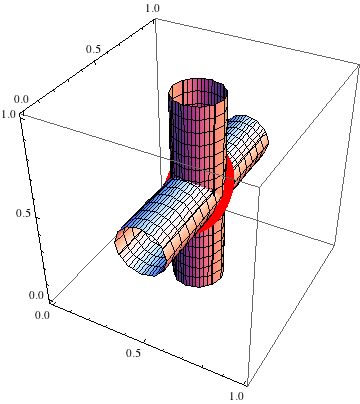
\includegraphics[width=0.5\textwidth]{imgs/cylinder_model_planeless.png}
  %\vspace{1mm}
  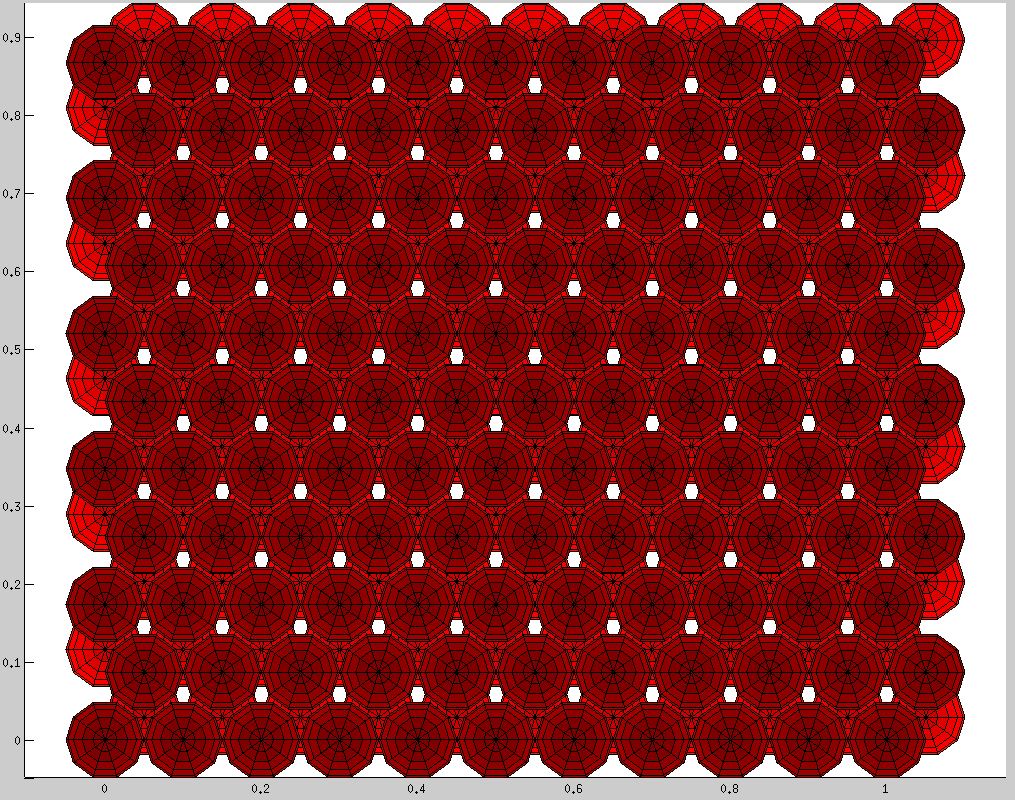
\includegraphics[width=0.5\textwidth]{imgs/packedSpheres.png}
  
  \vspace{5mm}
  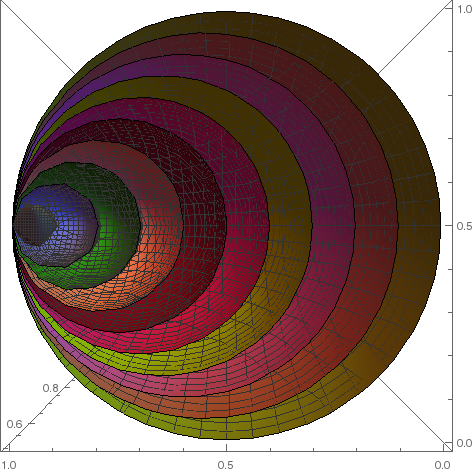
\includegraphics[width=0.5\textwidth]{imgs/hardEllipsoidsSingle.png}
  \caption{Test Scenes, from Top to Bottom:
    %{\bf Test Cylinders};
    {\bf Packed Spheres};
    {\bf Shifted Ellipsoids}}
  \label{fig:testScenes}
\end{figure}

\subsection{Analysis}
To analyze the results, we computed the least squares linear fit of
the timing data.  For the Packed Ellipsoids, we used the number of
comparisons made as our independent variable, and computed a linear
coefficient for it along with a constant term.  For the set of Shifted
Ellipsoids, we were able to aggregate the test results for each type
of scene.  This allowed us to fit the line to two independent
variables; the number of comparisons made, and the number of quadric
surfaces in the scene.  Fitting the time it takes to make a comparison
to a linear relationship makes sense, as the bulk of the sorting time
is taken up by performing these comparisons.  It also makes sense for
the time to be linearly related to the number of quadrics in the
scene, as the cached values are only computed once for each quadric,
and are likely to significantly affect the time a comparison takes.

\subsection{Hardware}
Three computers were used to test the implementations.  The first
computer has a Core i3 M370 processor with 2 cores and a 3 MB cache.
This processor does provide not a hardware implementation of FMA.
This computer has 4 GB of DDR3 memory clocked at 1 GHz.  It is running
an up to date installation of Arch Linux with version 4.4 of the
kernel.  GCC 5.3 was used to compile the code for these tests.  For
these tests, the performance manager was set to keep the CPU clock at
2.4 GHz, and the process was run with a nice value of -20.

The second computer has two Xeon E5-2643 processors with 4 cores and
10 MB caches.  This processor does not provide a hardware
implementation of FMA.  This computer has 32 GB of DDR3 memory running
with a 1.6 GHz clock.  It is running Ubuntu 14.04 with version 3.13 of
the kernel, and uses GCC 5.2 to compile the code for these tests.
These tests were run with the default performance manager with a
maximum CPU clock of 3.3 GHz, along with a nice value of -20.

The third computer has a Core 2 Duo E6550 processor with two cores and
a 4 MB cache.  This processor does not provide a hardware
implementation of FMA.  This computer has 8 GB of DDR2 memory clocked
at 667 MHz.  It is running an up to date installation of Gentoo Linux
with version 4.0 of the kernel.  GCC 5.3 was used to compile the code
for these tests.  For these tests, the performance manager was set to
keep the CPU clock at 2.3 GHz, with a nice value of -20.

To get a better estimate of the relative performance of the two
computers, the Geekbench benchmark was employed to estimate the
processor speeds.  The Ubuntu computer had a single core floating
point score of 2730.  The Arch computer had a single core floating
point score of 1702.  The Gentoo computer had a single core floating
point score of 1408.  On average, the Ubuntu computer was capable of
about 1.6 times more FLOPS than the Arch computer, and 1.9 times more
FLOPS than the Gentoo computer.

\section{Experimental Results}
The results of the experiments are shown in Table \ref{tab:times}.
Each method took approximately the same amount of time to process each
quadric, though the resultant method consistently took the longest.
This is because the resultant method caches some of the intermediate
values when the first comparison is made, shifting some portion of the
cost from the ms/Comp term to the ms/Quadric term.  The
amount that is shifted is determined by how many quadrics a random
line can be expected to intersect, and how many ambiguous orderings a
single line-quadric intersection will be involved in.  The increased
precision approximation method also took longer than the machine
precision approximation method for essentially the same reason as the
resultant method.  It's not entirely clear why it took less time than
the resultant method, as it performs harder computations on the first
use of the quadrics roots than the resultant.

The second term is approximately how much time each comparison takes.
Not surprisingly, the machine precision method took very little time
per comparison.  This is because nearly all of it's work is done on a
per quadric basis - the roots are calculated for each quadric once,
and only a subtraction is required for each comparison. The resultant
method also performed significantly better than the increased
precision method on a per comparison basis.  This is as expected,
given the reduction in the amount of precision, the number of FLOPs
required, and the lack of operations such as square roots and
divisions.

The constant term appears to be rather meaningless when we measure the
ms/Quadric term.  This is good, because it shows that when the
ms/Quadric term is not measured, that is mainly what the constant term
consists of.  Thus, we expect, and observe the same results as in the
ms/Quadric term.  It also means there are probably not any other terms
which should be considered.

\begin{figure}
  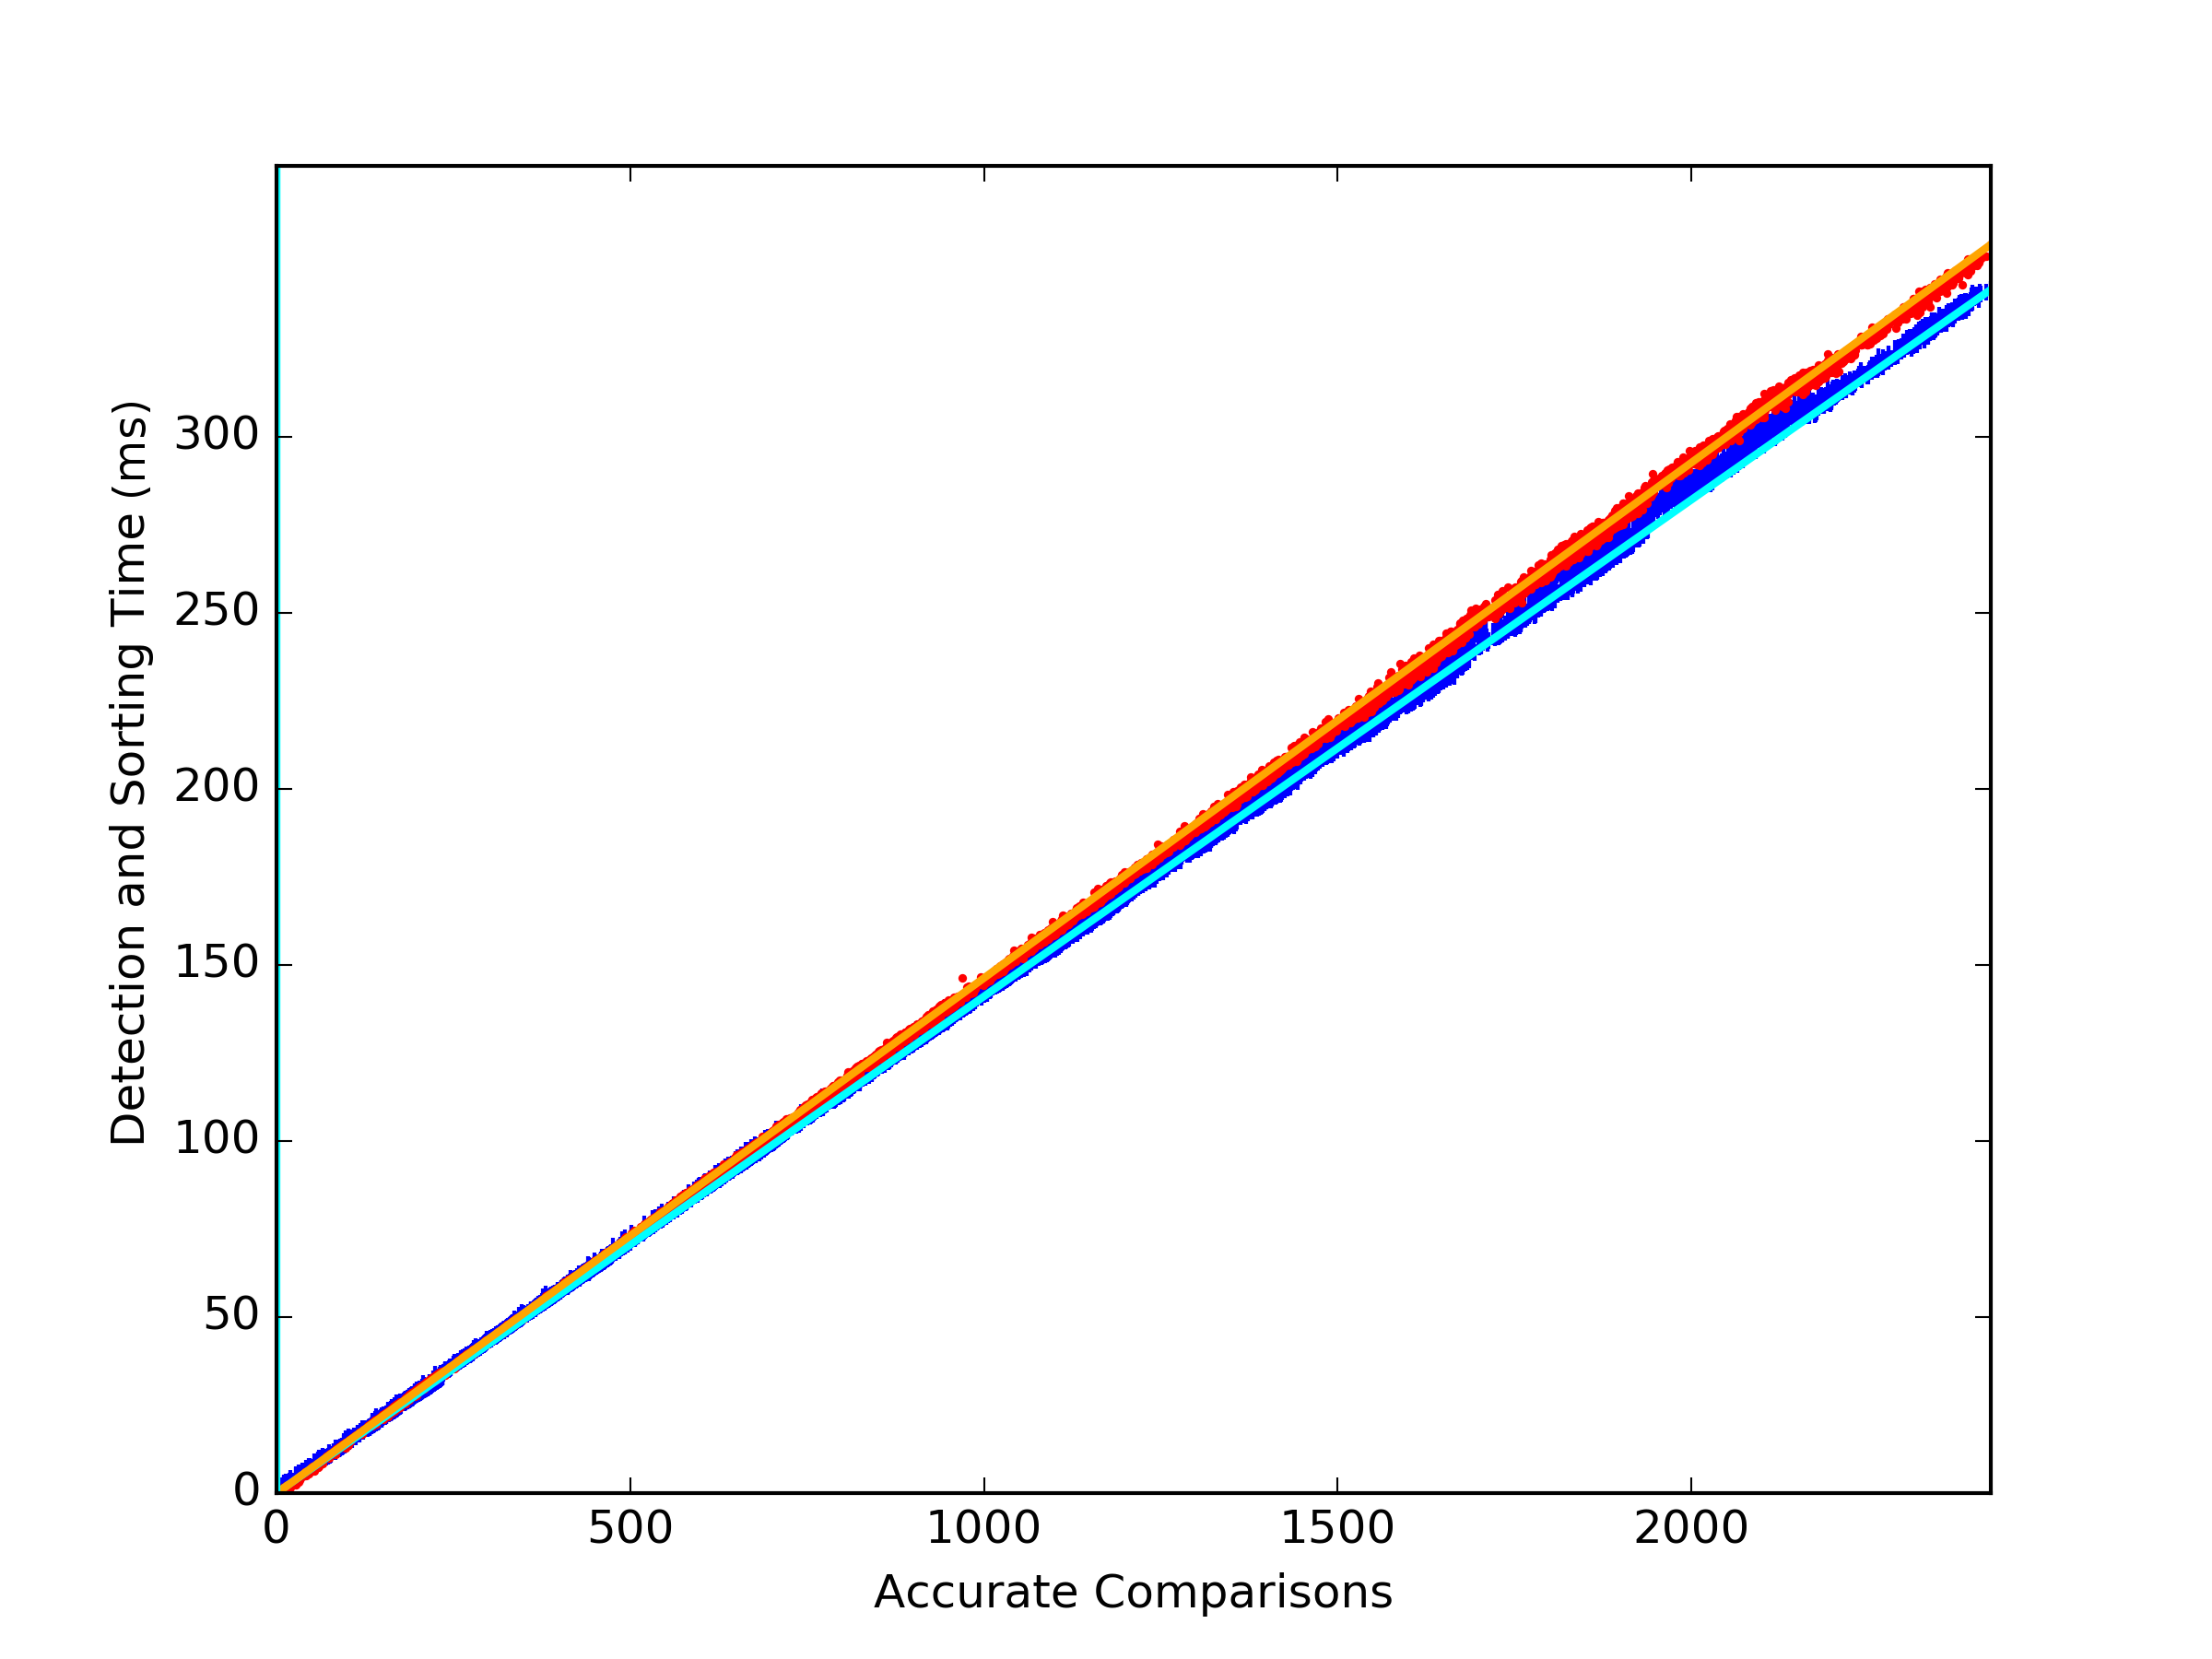
\includegraphics[width=0.55\textwidth]{imgs/hardEllipsoidsSingle_gentoo_adjusted.png}
  \caption{Typical plot of Number of Comparisons vs. the Evaluation
    Time (ms); {\bf Red: Approximation Method at $24\times$ the
      Input Precision}; {\bf Green: Approximation Method at Input Precision}; {\bf Blue: Resultant Method}}
  \label{fig:linefit}
\end{figure}

Figure \ref{fig:linefit} shows a plot of the results from one of the
tests.  It appears to confirm our expectation that the time required
is linearly coorelated with the number of precision increases.

\begin{table}[p]
  \captionsetup{oneside, margin={1cm,0cm}, width=\textwidth}
  \caption{Timing Results of the Approximate Comparison and Resultant Comparison}
  \label{tab:times}
  \begin{tabular}{|l|l|ll|lll|l|}
\hline
Machine & Scene & Method & Disagreements & $\frac{\text{ms}}{\text{Quadric}}$ & $\frac{\text{ms}}{\text{Comparison}}$ & Constant $\text{ms}$ & Residual ($\text{ms}^2$)\\
\hhline{|=|=|==|===|=|}
Ubuntu & Packed & Increased Prec. & \hphantom{1}--- & -- & \hphantom{-}0.06823 & \hphantom{-}5.399 & \hphantom{10}1194.8288\\
& Spheres & Approximate & 103 & -- & -0.009685 & \hphantom{-}5.399 & \hphantom{10}1161.2192\\
&& Resultant & \hphantom{1}89 & -- & \hphantom{-}0.05687 & \hphantom{-}5.408 & \hphantom{10}1194.1208\\
\hline
& Nested & Increased Prec. & \hphantom{1}--- & 0.004163 & \hphantom{-}0.07064 & -0.002835 & \hphantom{1}28554.479\\
& Spheres & Approximate & \hphantom{1}13 & 0.004098 & \hphantom{-}0.000255 & -0.001070 & \hphantom{10}2806.9520\\
&& Resultant & \hphantom{10}0 & 0.004309 & \hphantom{-}0.05846 & \hphantom{-}0.007079 & \hphantom{1}32989.590\\
\hline
Arch & Packed & Increased Prec. & \hphantom{1}--- & -- & \hphantom{-}0.1364 & \hphantom{-}4.893 & \hphantom{100}334.98312\\
& Spheres & Approximate & \hphantom{1}85 & -- & \hphantom{-}0.000304 & \hphantom{-}4.942 & \hphantom{100}316.04740\\
&& Resultant & \hphantom{1}75 & -- & \hphantom{-}0.1139 & \hphantom{-}4.921 & \hphantom{100}327.24112\\
\hline
& Nested & Increased Prec. & \hphantom{1}--- & 0.003835 & \hphantom{-}0.1157 & \hphantom{-}0.05856 & 582387.69\\
& Spheres & Approximate & \hphantom{1}11 & 0.003864 & \hphantom{-}0.000591 & -0.01970 & \hphantom{10}7533.7867\\
&& Resultant & \hphantom{10}1 & 0.004088 & \hphantom{-}0.09580 & \hphantom{-}0.05074 & 558251.79\\
\hline
Gentoo & Packed & Increased Prec. & \hphantom{1}--- & -- & \hphantom{-}0.1711 & \hphantom{-}4.522 & \hphantom{100}255.93646\\
& Spheres & Approximate & \hphantom{1}94 & -- & \hphantom{-}0.004651 & \hphantom{-}4.513 & \hphantom{100}256.48723\\
&& Resultant & \hphantom{1}84 & -- & \hphantom{-}0.1424 & \hphantom{-}4.551 & \hphantom{100}258.49985\\
\hline
& Nested & Increased Prec. & \hphantom{1}--- & 0.003670 & \hphantom{-}0.1639 & \hphantom{-}0.02020 & \hphantom{1}62122.965\\
& Spheres & Approximate & \hphantom{1}19 & 0.003562 & \hphantom{-}0.000446 & -0.003482 & \hphantom{10}3327.8361\\
&& Resultant & \hphantom{10}0 & 0.003892 & \hphantom{-}0.1372 & \hphantom{-}0.06507 & 176409.02\\
\hline
\end{tabular}

\end{table}

\section{Conclusion}
In this paper we showed how the resultant method can improve the
accuracy in comparing a single line-quadric intersections at a much
lower cost than simply increasing the amount of precision.  This
method also satisfies our notion of correctness, unlike the
approximation method.  This method is applicable in many cases and can
provide significant improvements to performance over the regular
method of increasing precision.

A remaining problem to solve is computing the intersection order
correctly when the order of mutliple roots is undetermined.  When a
shared root is detected, it would be easy to determine if the other
roots are shared as well with the discriminants.  Because the terms of
the discriminants are fast to compute exactly, they could be compared
exactly relatively easily.  Since the discriminant is quadratically
related to the distance between the roots of a polynomial, this will
tell us exactly if both roots are shared, and if not, the order of the
non-shared roots.

\section{Acknowledgment}
We thank David Griesheimer for discussions on this problem, and both NSF and Bettis Labs for their support of this research. 

\bibliographystyle{plain}
\bibliography{resultantmethod}
\end{document}
